\chapter{Lecture 17 - Numeric Differentiation with Finite Difference Formulas}
\label{ch:lec17n}
\section{Objectives}
The objectives of this lecture are to:
\begin{itemize}
\item Derive basic differentiation formulas using Taylor series expansions.
\item Express the differentiation operation in matrix form.
\end{itemize}
\setcounter{lstannotation}{0}

\section{Introduction}
Numeric differentiation plays an important role in scientific computing.  In the last lecture, we learned to use interpolation to visualize the temperature distribution on a surface as computed in a FEM-based analysis.  Suppose we wanted also to calculate the heat flux along a boundary of the domain?  As was discussed in the analytic methods portion of this text, the heat flux is related to the derivative of the temperature field:
\begin{equation*}
q^{\prime \prime} = -k \nabla T
\end{equation*}
where $k$ is the thermal conductivity.  In one spatial dimension, this simplifies to: $q^{\prime \prime} = -k \sfrac{dT}{dx}$.
In this lecture we will discuss methods for estimating derivatives of a function, $f(x)$, where the function is represented as a vector.  This family of methods is referred to as \emph{finite difference} methods.

\begin{marginfigure}
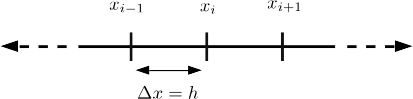
\includegraphics{lec17n-dx.png}
\caption{A discrete grid on which a function may be defined.}
\label{fig:lec17n-dx}
\end{marginfigure}
\section{First Derivative}
Consider a function defined on a discrete grid as shown in Figure \ref{fig:lec17n-dx}.  For simplicity of the following analysis, we will assume that the grid points are all equally spaced: $\Delta x = h$.  Suppose we know the value of the function,$f(x_i)$, at all grid points, $x_i$, and we wish to estimate the first derivative, $f^{\prime}(x_i)$.  From the Taylor series expansion we have:
\begin{multline*}
f(x_{i+1}) = f(x_i) + f^{\prime}(x_i)\overbrace{(x_{i+1}-x_i)}^{h} + \frac{f^{\prime \prime}(x_i)}{2!}\overbrace{(x_{i+1} - x_i)^2}^{h^2} + \cdots + \\ \frac{f^{(n)}(x_i)}{n!}\overbrace{(x_{i+1}-x_i)^n}^{h^n} + \cdots
\end{multline*}
If we solve for $f^{\prime}(x_i)$, we obtain a two-point \emph{forward difference} formula:
\begin{align*}
f^{\prime}(x_i) &= \frac{f(x_{i+1}) - f(x_i)}{h} - \text{higher order terms} \\
f^{\prime}(x_i) &= \frac{f(x_{i+1}) - f(x_i)}{h} - \frac{f^{\prime \prime}(\xi)}{2!}h
\end{align*}
in which it can be shown that the higher order terms are equal to $\frac{f^{\prime \prime}(\xi)}{2!}h$ with $\xi \in [x_{i},x_{i+1}]$.  We can more generically characterize that error term using asymptotic notation: $\mathcal{O}(h)$.

We can similarly define a two-point backward difference formula:
\begin{align*}
f(x_{i-1}) &= f(x_i) - f^{\prime}(x_i)h + \frac{f^{\prime \prime}(x_i)}{2!}h^2 - \cdots \\
\Rightarrow f^{\prime}(x_{i}) &= \frac{f(x_i) - f(x_{i-1})}{h} + \mathcal{O}(h)
\end{align*}
These equations are simple to use and effective, however they have a significant drawback in that the error term is proportional to $h$.  For every extra decimal place we need to gain in accuracy, we must to reduce $h$ by a factor of 10.  This adds up quickly.  The good news is that we can do better.  

For first derivative formulas, we can try a centered difference scheme:\marginnote{


\vspace{2.3cm} 

\noindent Here we subtract the first equation from the second and solve for $f^{\prime}(x_i)$.
}
\begin{align*}
f(x_{i+1}) &= f(x_i) + f^{\prime}(x_i)h + \frac{f^{\prime \prime}(x_i)}{2!}h^2 + \mathcal{O}(h^3) \\
f(x_{i-1}) &= f(x_i) - f^{\prime}(x_i)h + \frac{f^{\prime \prime}(x_i)}{2!}h^2 - \mathcal{O}(h^3) \\
f^{\prime}(x_i) &= \frac{f(x_{i+1})- f(x_{i-1})}{2h} + \underbrace{\frac{\mathcal{O}(h^3)}{2h}}_{\mathcal{O}(h^2)}
\end{align*}
This results in second-order convergence.  We can also get second-order convergence if we use more data points in the derivation.  We will skip the messy algebraic details but three-point, second-order forward and backward differentiation formulas are given in Equation \ref{eq:lec17n-fdf}, and Equation \ref{eq:lec17n-bdf}.

\begin{equation}
f^{\prime}(x_{i}) = \frac{-3f(x_i) + 4f(x_{i+1}) - f(x_{i+2})}{2h}
\label{eq:lec17n-fdf}
\end{equation}

\begin{equation}
f^{\prime}(x_{i}) = \frac{f(x_{i-2}) - 4f(x_{i-1}) + 3f(x_i)}{2h}
\label{eq:lec17n-bdf}
\end{equation}

\vspace{0.5cm}

\noindent\textbf{Example: } Use the 2- and 3-point finite difference formulas to numerically differentiate $\cos{x}$.  

\vspace{0.1cm}

\noindent In this listing, we carry out the differentiation with 2-point difference methods. \marginnote[8.0cm]{

\noindent \ref{lst:ann17n-1} here we use these vectors to index \lstinline[style=myMatlab]{df_numeric} and \lstinline[style=myMatlab]{f} in a ``vectorized'' fashion rather than one equation at a time.
}
\begin{lstlisting}[style=myMatlab,name=lec17n-ex1]
clear
clc
close 'all'

f = @(x) cos(x);

n = 7;
Nx = 2^n;
xMin = 0; xMax = pi;
X = linspace(xMin,xMax,Nx);
h = X(2) - X(1);

% initialize the derivative array
df_numeric = nan(1,Nx); 

% use fwd difference at left end
df_numeric(1) = (1/h)*(f(X(2))- f(X(1)));

% use backward difference at right end
df_numeric(end) = (1/h)*(f(X(end)) - f(X(end-1)));

% use centered difference everywhere else
i = 2:(Nx-1); ip = i+1; im = i-1; /*!\annotation{lst:ann17n-1}!*/
df_numeric(2:(end-1)) = (1/(2*h))*(f(X(ip))-f(X(im)));

% plot the function and its derivative
Xp = linspace(xMin,xMax,10000);
figure(1)
plot(Xp,f(Xp),'-b',...
    X,df_numeric,'-r','linewidth',2);
grid on;
title('First Derivative of $\cos{x}$',...
    'fontsize',14,...
    'fontweight','bold','Interpreter','latex');
xlabel('X','fontsize',12,'fontweight','bold');
ylabel('Y','fontsize',12,'fontweight','bold');
legend('f(x)','f^{\prime}(x)');
set(gca,'fontsize',12,'fontweight','bold');
\end{lstlisting}
\begin{marginfigure}
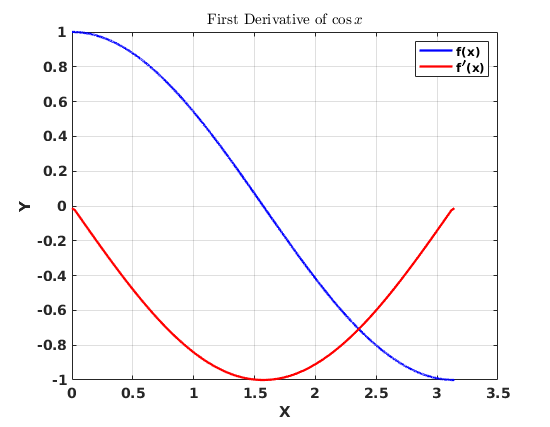
\includegraphics{lec17n-ex1-first-deriv.png}
\caption{A plot of $cos{x}$ and its first derivative calculated numerically.}
\label{fig:lec17n-ex1-first-deriv}
\end{marginfigure}

In the next listing a method for carrying out a convergence analysis is shown.
\begin{lstlisting}[style=myMatlab,name=lec17n-ex1]
%% Get Convergence Rate
N = 5:15;
rel_err = nan(1,length(N));
h_err = nan(1,length(N));

for s = 1:length(N)
    Nx = 2^N(s);
    xMin = 0; xMax = pi;
    X = linspace(xMin,xMax,Nx);
    h = X(2) - X(1);
    h_err(s) = h;
    
    df_numeric = nan(1,Nx);
    % use fwd difference at left end
    df_numeric(1) = (1/h)*(f(X(2))- f(X(1)));
    % use backward difference at right end
    df_numeric(end) = (1/h)*(f(X(end)) - f(X(end-1)));
    % use centered difference everywhere else
    i = 2:(Nx-1); ip = i+1; im = i-1;
    df_numeric(i) = (1/(2*h))*(f(X(ip))-f(X(im)));
    
    % estimate the relative error
    x_err = 1:Nx; % include the end points
    %x_err = 2:(Nx-1); % exclude the end points
   
    rel_err(s) = norm(df_numeric(x_err) - df(X(x_err)),2)...
        /norm(df(X(x_err)),2);    
end

% add gauge lines for convergence
c1 = 0;
h1 = h_err + c1;

c2 = 0;
h2 = h_err.^2 + c2;

figure(2)
loglog(h_err,rel_err,'-b',...
    h_err,h1,'--r',...
    h_err,h2,'--g','linewidth',3);
title('Convergence Behavior','fontsize',14,...
    'fontweight','bold');
xlabel('h','fontsize',12,'fontweight','bold');
ylabel('Relative Error','fontsize',12,'fontweight','bold');
grid on
set(gca,'fontsize',10,'fontweight','bold');
legend('Estimate','h^1 convergence','h^2 convergence',...
    'location','best');
\end{lstlisting}
We use the 2\textsuperscript{nd}-order accurate centered difference equation through most of the domain but, as Figure \ref{fig:lec17n-ex1-first-deriv-convergence} shows, the first-order accurate 2-point formulas at the end-points are enough to spoil convergence.

\begin{marginfigure}[-10.0cm]
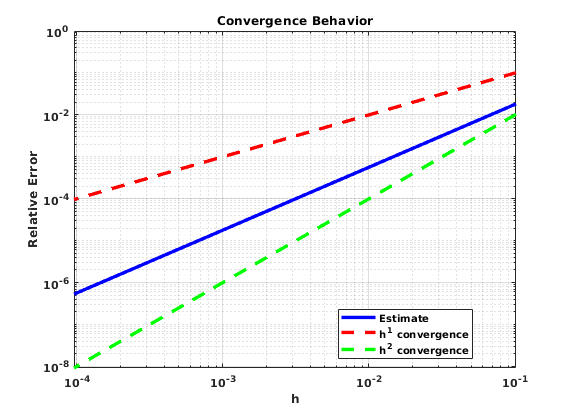
\includegraphics{lec17n-ex1-first-deriv-convergence.png}
\caption{Convergence behavior using 2-point finite difference formulas.}
\label{fig:lec17n-ex1-first-deriv-convergence}
\end{marginfigure}

If we use the 2\textsuperscript{nd}-order 3-point forward and backward differentiation formulas, we can get convergence at 2\textsuperscript{nd}-order as shown in Figure \ref{fig:lec17n-ex1-first-deriv-convergence2}.

\begin{marginfigure}[-3.0cm]
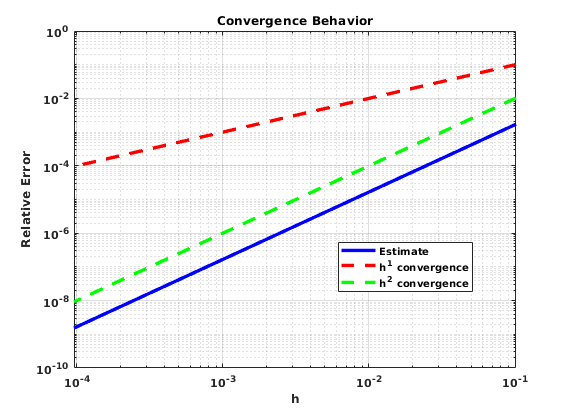
\includegraphics{lec17n-ex1-first-deriv-convergence2.png}
\caption{Convergence behavior using 2\textsuperscript{nd}-order finite difference equations throughout the domain.}
\label{fig:lec17n-ex1-first-deriv-convergence2}
\end{marginfigure}

\section{Second Derivative Formulas}

We can use finite difference equations to approximate the second derivative (and higher-order derivatives) as well.  As with first-order differentiation, we derive the formula from Taylor-series expansion.

\begin{align*}
f(x_{i+1})=f(x_i)+f^{\prime}(x_i)h+\frac{f^{\prime \prime}(x_i)h^2}{2!}+\frac{f^{\prime\prime\prime}(x_i)h^3}{3!}+ \cdots \\
f(x_{i-1})=f(x_i)-f^{\prime}(x_i)h+\frac{f^{\prime \prime}(x_i)h^2}{2!}-\frac{f^{\prime\prime\prime}(x_i)h^3}{3!}+ \cdots
\end{align*}
If we add the two equations above and solve for $f^{\prime \prime}(x_i)$, we get:
\begin{equation}
f^{\prime \prime}(x_i) = \frac{2f(x_{i-1})-2f(x_{i})+f(x_{i+1})}{h^2}+\mathcal{O}(h^2)
\label{eq:secondDeriv-centered}
\end{equation}

Through a similar process, second-order accurate forward- and backward-differentiation formulas can be derived for use at domain end-points:
\begin{equation}
f^{\prime \prime} = \frac{2f(x_i) - 5f(x_{i+1}) + 4f(x_{i+2}) - f(x_{i+3})}{h^2} 
\label{eq:secondDeriv-forward}
\end{equation}

\begin{equation}
f^{\prime \prime} = \frac{-f(x_{i-3})+4f(x_{i-2})-5f(x_{i-1})+2f(x_i)}{h^2} 
\label{eq:secondDeriv-backward}
\end{equation}


\section{Representation as a Matrix}
It is convenient to represent finite difference equations as a matrix.  For example, to take the first derivative of a function, $f(x)$, that is represented by a vector $f$ that samples $f(x)$ at uniformly spaced points, the 2nd-order finite difference equations would be:
\begin{align*}
\frac{1}{2h}\left[-3f(x_1)+4f(x_2)-f(x_3)\right] &= f^{\prime}(x_1) \\
\frac{1}{2h}\left[-f(x_1) + f(x_3) \right] &= f^{\prime}(x_2) \\
\frac{1}{2h}\left[-f(x_2) + f(x_4) \right] &= f^{\prime}(x_3) \\
\qquad \vdots \qquad &= \qquad \vdots \qquad \\
\frac{1}{2h}\left[-f(x_{n-2} + f(x_{n})\right] &= f^{\prime}(x_{n-1}) \\
\frac{1}{2h}\left[f(x_{n-2} - 4f(x_{n-1}) + 3f(x_{n}) \right]&=f^{\prime}(x_n)
\end{align*}
where $h$ is the distance between the points, $h=x_i - x_{i-1}$.  These equations can be represented in matrix-vector notation as:
\begin{equation*}
\frac{1}{2h}\bracketMatrixstack{
-3 & 4 & -1 & 0 & 0 & 0 & \cdots & 0\\
-1 & 0 & 1 & 0 & 0 & 0 & \cdots & 0\\
0 & -1 & 0 & 1 & 0 &  0 & \cdots & 0\\
0 & 0 & -1 & 0 & 1 & 0 & \cdots & 0 \\
\vdots & \ddots & \ddots & \ddots & \ddots & \ddots & \ddots & \vdots \\
0 & 0& \cdots & 0 & -1 & 0 & 1 & 0 \\
0 & 0 & \cdots & \cdots & 0 & -1 & 0 & 1 \\
0 & 0 & \cdots & \cdots & 0 & -1 & -4 & 3 
}
\bracketVectorstack{
f(x_1) \\
f(x_2) \\
f(x_3) \\
f(x_4) \\
\vdots  \\
f(x_{n-2}) \\
f(x_{n-1}) \\
f(x_{n})
}
=
\bracketVectorstack{
f^{\prime}(x_1) \\
f^{\prime}(x_2) \\
f^{\prime}(x_3) \\
f^{\prime}(x_4) \\
\vdots  \\
f^{\prime}(x_{n-2}) \\
f^{\prime}(x_{n-1}) \\
f^{\prime}(x_n)
}
\end{equation*}
Or, more concisely:
\begin{equation*}
Af = f^{\prime}
\end{equation*}
where $A$ is a sparse $n \times n$ matrix of the coefficients.  The matrix $A$ should be thought of as a discrete representation of the differentiation operator.  Whereas in calculus class one might write:
\begin{equation*}
\frac{d}{dx}f(x) = f^{\prime}(x)
\end{equation*}
The discrete version of this is given in the equation above.  The functions have been replaced by vectors and the differential operator has been replaced by a matrix which their respective discrete equivalents. Of course, the matrix/vector formulation is an approximation, but the approximation improves as $h$ is reduced.

\vspace{0.2cm}

\noindent\textbf{Example:} Consider the boundary value problem below:
\begin{align*}
\frac{d^2f}{dx^2} + \lambda^2 f &= 0, \ \ \lambda>0, \ 0<x<\pi \\
f(0) = 0, \ f(\pi) &= 0
\end{align*}
The general solution to the differential equation is:
\begin{equation*}
f(x) = c_1 \cos{(\lambda x)}+c_2\sin{(\lambda x)} 
\end{equation*}
The boundary condition at $x=0$ gives us:
\begin{equation*}
f(0) = c_1 \cancelto{1}{\cos{(0)}} + c_2 \cancelto{0}{\sin{(0)}} = 0 \ \Rightarrow c_1 = 0
\end{equation*}
For the boundary condition at $x = \pi$ we have:
\begin{equation*}
f(\pi) = c_2 \sin{(\lambda \pi)} = 0
\end{equation*}
As usual, we are looking for non-trivial solutions, so rather than set $c_2 = 0$, we look for values of $\lambda$ such that $\sin{(\lambda \pi)} = 0$. This will be true when $\lambda \pi = n \pi$ where $n$ is a positive integer.\marginnote{\textbf{Note:} We exclude the case $n=0$ since we stipulated that $\lambda > 0$.} Thus, $\lambda = n$, so the eigenvalues are $\lambda^2 = n^2$ for $n=1,2,3,\dots$, and the eigenfunctions are:
\begin{equation}
f_n(x) = \sin{nx}
\label{eq:lec17n-ex2-eigenfunctions}
\end{equation}
We can solve the same eigenvalue problem using differentiation matrices.  Applying the finite difference equations given in Equations \ref{eq:secondDeriv-centered},\ref{eq:secondDeriv-forward} and \ref{eq:secondDeriv-backward}, we can assemble a matrix representation of the differential operator:\marginnote{\textbf{Note:} As can be seen, it is really more correct to say that the eigenvalues are $-\lambda^2=n^2$ or $-1,-4,-9,\dots$}
\begin{align*}
\frac{d^2f}{dx^2} &= -\lambda^2 f \\
Af &= -\lambda^2 f
\end{align*}
This is accomplished in the code block below:
\begin{lstlisting}[style=myMatlab,name=lec17n-ex2]
% discretize the spatial domain
N = 9;
Nx = 2^N;
xMin = 0; xMax = pi;
X = linspace(xMin,xMax,Nx);
h = X(2) - X(1);

% Create a matrix for 2nd derivative operator
A = zeros(Nx,Nx); 

% set coefficients for first equation
A(1,1) = 2/h^2; A(1,2) = -5/h^2;
A(1,3) = 4/h^2; A(1,4) = -1/h^2;

% set coefficents for all interior equations
for m=2:(Nx-1)
    A(m,m) = -2/h^2; A(m,m-1) = 1/h^2;
    A(m,m+1) = 1/h^2;
end

% set coefficents for last equation
A(Nx,Nx) = 2/h^2; A(Nx,Nx-1) = -5/h^2;
A(Nx,Nx-2) = 4/h^2; A(Nx,Nx-3) = -1/h^2;
\end{lstlisting}

We need to apply the boundary conditions to the matrix A.  One way of accomplishing this is illustrated in the next code block.\marginnote{
\ref{lst:ann17n2-1} Here we set the first and last diagonal of $A$ to 1; the first and last row and column, other than the diagonal, is set to zero.  Effectively this eliminates the first and last equation of $A$ from the matrix.  This method of applying the Dirichlet boundary condition has the feature that the symmetry of $A$ is preserved.  
}
\begin{lstlisting}[style=myMatlab,name=lec17n-ex2]
% Set boundary conditions 
A(1,:) = 0; A(:,1) = 0; A(1,1) = 1; /*!\annotation{lst:ann17n2-1}!*/
A(end,:) = 0; A(:,end) = 0; A(end,end) = 1;
\end{lstlisting}

We will use the MATLAB built-in function \lstinline[style=myMatlab]{eigs} to find the eigenvalues and eigenvectors of $A$ 

\begin{lstlisting}[style=myMatlab,name=lec17n-ex2]
%  Get the four smallest eigenvalues and eigenvectors of A
[V,D] = eigs(A(2:(end-1),2:(end-1)),4,'smallestabs');

% reduce the X domain to exclude the boundaries
X_red = X(2:(end-1));
figure(5)

subplot(4,1,1)
plot(X_red,(V(:,1))/norm(V(:,1),2),'.b')
title('First Four Eigenvectors of A',...
    'FontSize',14,'FontWeight','bold');
subplot(4,1,2)
plot(X_red,(V(:,2))/norm(V(:,2),2),'.b')

subplot(4,1,3)
plot(X_red,(V(:,3))/norm(V(:,3),2),'.b')

subplot(4,1,4)
plot(X_red,(V(:,4))/norm(V(:,4),2),'.b')
xlabel('X','FontSize',12,'FontWeight','bold');

% Display the eigenvalues
fprintf('D = \n');
disp(D);
\end{lstlisting}
\begin{marginfigure}
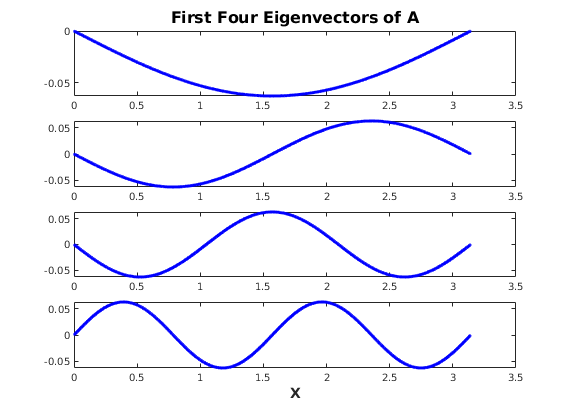
\includegraphics{lec17n-ex2-eigenvectors.png}
\caption{A plot of the first four eigenvectors of $A$.}
\label{fig:lec17n-ex2-eigenvectors}
\end{marginfigure}
\begin{marginfigure}
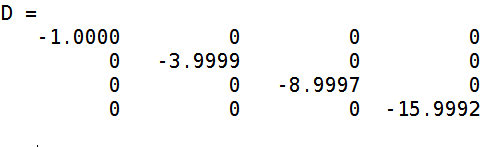
\includegraphics{lec17n-ex2-eigenvalues.png}
\caption{The matrix $D$ with the first 4 eigenvalues of $A$.}
\label{fig:lec17n-ex2-eigenvalues}
\end{marginfigure}
The first four eigenvectors of $A$ are plotted in Figure \ref{fig:lec17n-ex2-eigenvectors}. While not a rigorous proof, you can check and see that the eigenvectors are orthogonal\sidenote{It is worth admitting here that the eigenvectors of \emph{all} symmetric matrices are orthogonal.  Since $A$ is symmetric, its eigenvectors are orthogonal. Still there is a deeper connection -- the differential operator that $A$ represents is, in some way, \emph{symmetric} and that is reflected in the symmetry of $A$.} which is analogous to the orthogonality of the eigenfunctions given in Equation \ref{eq:lec17n-ex2-eigenfunctions}. The eigenvalues are shown on the main diagonal of $D$ in Figure \ref{fig:lec17n-ex2-eigenvalues}.

